\documentclass{article}
\usepackage{graphicx}
\usepackage{amsmath}
\usepackage{enumerate}
\usepackage{amsfonts}

\begin{document}

\title{Lecture 0.3: Review of Trigonometry and Graphing Trigonometric Functions}
\author{Professor Leonard}
\maketitle

\section{Angles}

Plotting a vector and making an angle relative to the x-axis. The x-axis is called the
"initial side", the vector line is called the "terminal side".

Counter clockwise rotation from the x-axis gives positive angles. Clockwise gives negative
angles.

\subsection{Degrees vs. radians}
Radians involve $\pi$.\\

Coverting radians to degrees: 

\begin{align*}
    2\pi = 360^{\circ}\\
    f(x^{\circ}) = x^{\circ} \cdot \frac{\pi}{180^{\circ}}\\
    g(r) = r \cdot \frac{180^{\circ}}{\pi}
\end{align*}

$f(x^{\circ})$ converts degrees to radians. $g(r)$ converts radians to degrees.

He's going through some plotting of radian angles... not sure how to take notes on that. A
bit tricky, but if you have a radian (eg, $5\pi / 2$), then you take the four cartesian
quadrants, chop up the top and bottom halves equally by the denominator. The terminals of
the four axes end points are as follows (+$x$: 0 or $2\pi$, +$y$: $\pi/2$, -$x$: $\pi$,
-$y$: $3\pi/2$). And you then take the numerator coefficient and count that many either
counter clockwise (for positive numerator) or clockwise (for negative numerator).

\section{Trigonometric Functions}

Sine, cosine, and tangent are \emph{functions}. They need an input (usually an angle).
Sine, cosine, and tangent can be used to find the angles of a right triangle (remember
SohCahToa: sine, opposite over adjacent; cosine, adjacent over hypotenuse, tangent,
opposite over adjacent). \\

There's also the reciprocals of the three trig functions. 

\begin{align*}
    \text{Secant: } sec(\theta) = \frac{1}{cos(\theta)} = \frac{Hyp}{Adj}\\
    \text{Cosecant: } csc(\theta) = \frac{1}{sin(\theta)} = \frac{Hyp}{Opp}\\
    \text{Cotangent}: cot(\theta) = \frac{1}{tan(\theta)} = \frac{Adj}{Opp}
\end{align*}

For the unit circle (ie, circle with radius of 1), for any point $(x, y)$ along the
circumference of the circle, $cos(\theta)=x$, $sin(\theta) = y$, $tan(\theta) = y/x =
sin(\theta) / cos(\theta)$. And the reciprocal functions are just the reciprocals of these
outcomes.

\begin{center}
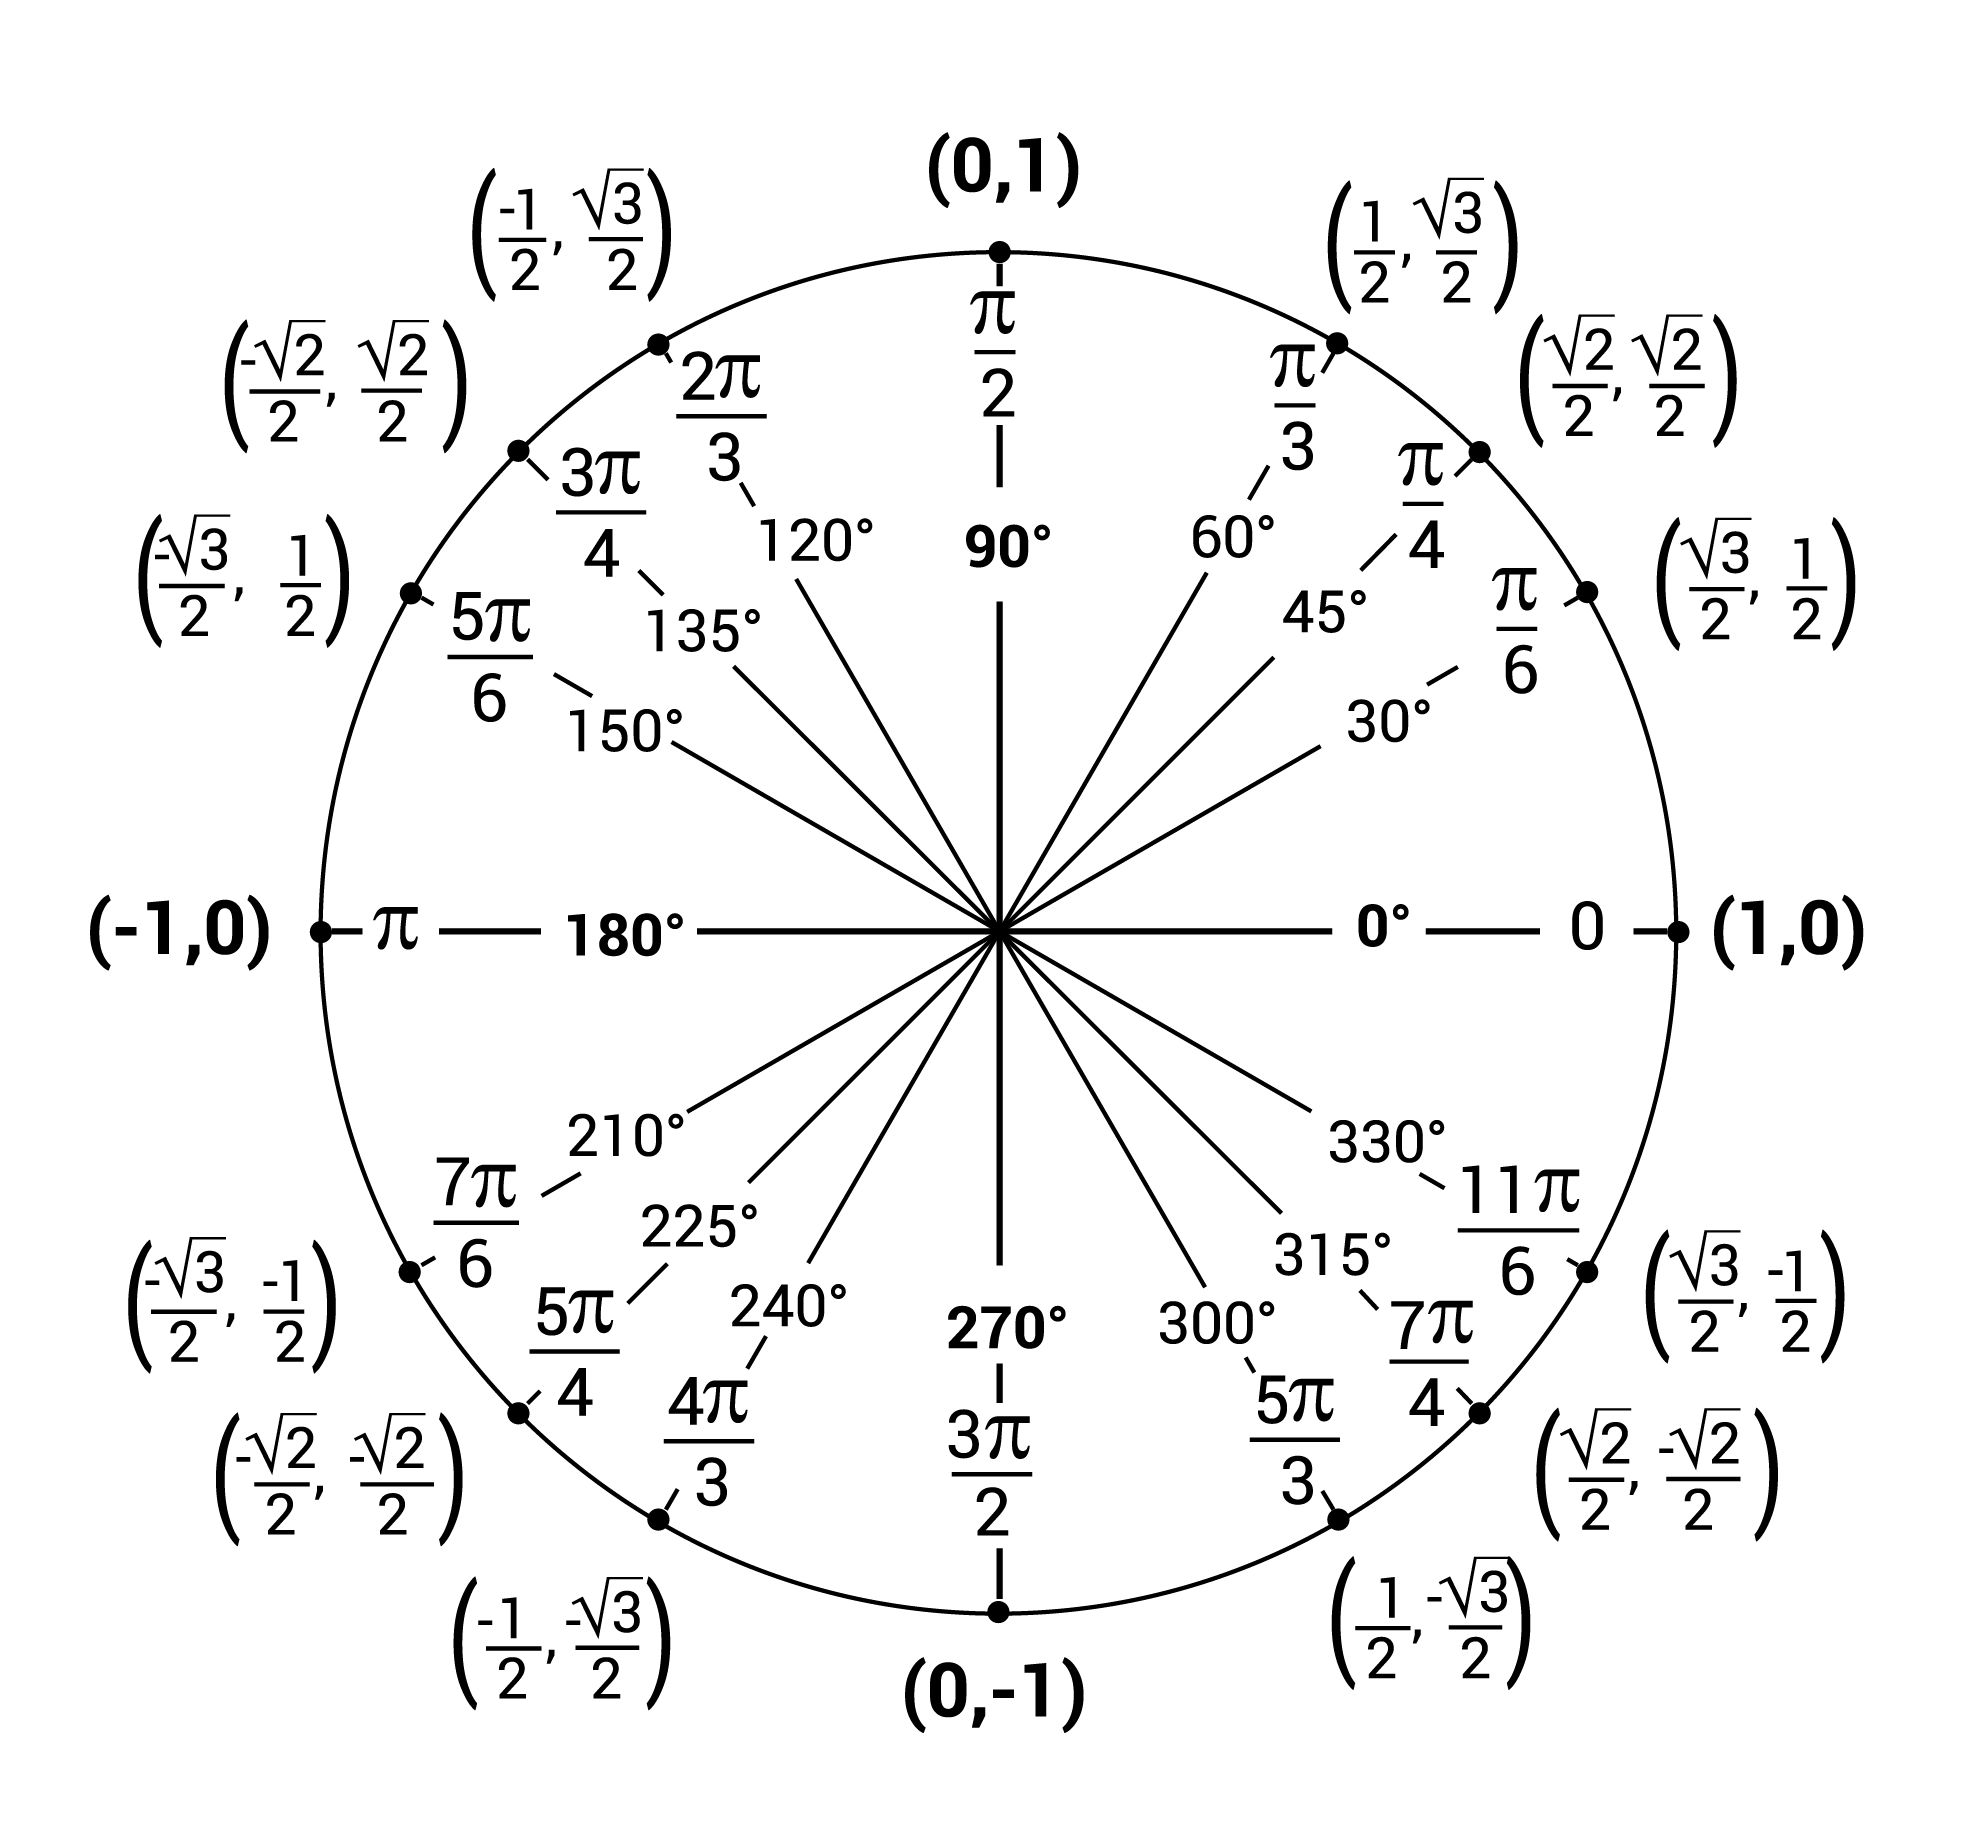
\includegraphics[scale=0.1]{Unit-circle.png}
\end{center}

He's stressing how important it is to know this unit circle. For example, one should know
the sin, cos, and tan of $\{0, \pi/2, \pi, 3\pi/2, 2\pi\}$. And should also know $\{\pi/3,
\pi/4, \pi/6\}$.

\subsection{Trigonometric functions across the quadrants}

Whether the trig functions are positive or negative depends on the quadrant. The mnemonic
"\textbf{A}ll \textbf{S}tudents \textbf{T}ake \textbf{C}alculus" $\rightarrow$ each letter
iterates through cartesian quadrants I:IV, A=All functions are positive in quadrant I,
S=Sine (and cosecant) is positive in quadrant II, T=Tangent (and cotangent) is positive in
quadrant III, C=Cosine (secant) is positive in quadrant IV. 


\subsection{Reference angles}

The idea is to make an acute angle with the x-axis, find the trig function of that, then
use the ASTC idea.\\

If the angle is already acute relative to x-axis, just take theta. Otherwise, find the
angle with x that makes it acute. So for example, if $\pi > \theta > 0$, then you
calculate the acute angle by $\pi - \theta$. Similar idea for quadrants III \& IV.

\subsection{Trig function for any angle}

One can use the properties of the functions across the quadrants and the reference angles,
along with knowledge of the unit circle, to determine for any input angle the output of
any trig function.\\

Example: find sin, cos, tan of $5\pi/3$.\\

Steps:
\begin{enumerate}
    \item Locate the quadrant.\\
        I think it's Quadrant IV\\
    \item Find the reference angle.\\
        $2\pi - 5\pi/3 = -3\pi / 3$\\
        Oh, fractions need a common denominator when adding or subtracting...\\
        $6\pi/3 - 5\pi/3 = \pi/3$\\
    \item Find all trig functions of the reference angle.\\
        I guess this is where we use the unit circle.\footnote{I had to take a little
            detour into the unit circle. Apparently the x y coordinates of the so-called
            "special angles/trianles" (30-60-90 and 45-45-90) are just givens and
            expressed as fractions of roots (so unsatisfying). So if want to find
            $sin(\pi/3)$ I have to go look up that the coordinates for the unit circle at
            $\theta = \pi/3$ are $(1/2, \sqrt{3}/2)$. Then obviously $sin(\pi/3) = y =
            \sqrt{3}/2$. And then you determine the sign of that by the quadrant.}
        
\end{enumerate}

\section{Graphing Trigonometric Functions}

We're going to graph things like this: $y = A \cdot sin(Bx)$ or $y = A \cdot cos(Bx)$. To
appreciate the impact of the coefficients, we'll compare $y = sin(x)$ against $y = 2 \cdot
sin(4x)$.

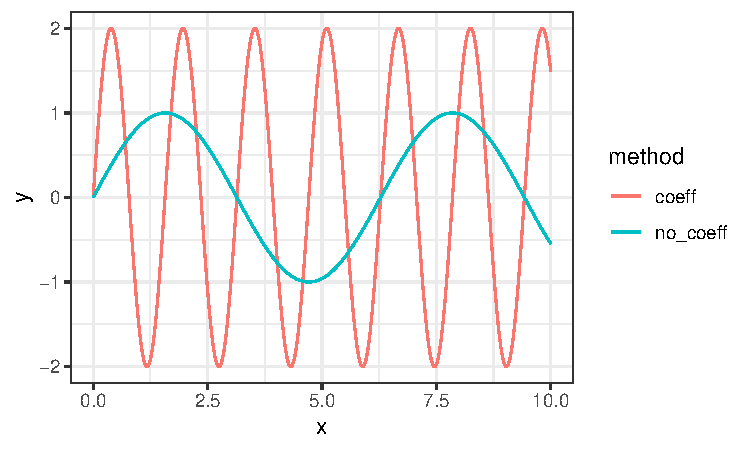
\includegraphics{fig1.pdf}

The period of a wave function is the stretch over which it's unique (ie, before it
repeats). \\

We get the amplitude and period by $\text{Amplitude} = \lvert A \rvert$ and $\text{Period}
= 2 \pi / B$.

You can break the period up into quarters to find the first positive and negative
amplitudes and the first x axis crossover point.

\subsection{Shifting the function}

Shifting the sin or cos function by a constant (ie, $y = A \cdot cos(Bx - c)$). Which is
rewritten as $y = A \cdot cos[B(x - c/b)]$. For reasons that aren't quite intuitive to me,
you flip the sign in terms of the shift---$-c/b$ is a shift to the right, and vice versa
for positive.

\textbf{Example:}

\begin{align*}
y = 3cos(2x + \frac{\pi}{2})\\
y = 3cos[2(x + \frac{\pi}{4})]\\
\text{Amplitude} = 3\\
\text{Period} = \frac{2\pi}{2}\\
\text{Period} = \pi\\
\text{Shift} = \frac{\pi}{4}
\end{align*}

You'll shift to the left by $\pi/4$.


In closing, he's saying you'll need to know trig identites (eg, $sin^2 + cos^2 = 1$, $tan
= sin/cos$). Half angle and double angle formulas ($sin(2x) = 2sin(x)cos(x)$). 

\end{document}

